% Name: Breadth-first search layers
% Description: A graph searched breadth first from s, drawn in layers by distance from s, with the search tree's edges solid and the rest dashed.
% Tags: BFS, breadth-first search, layers, graph traversal

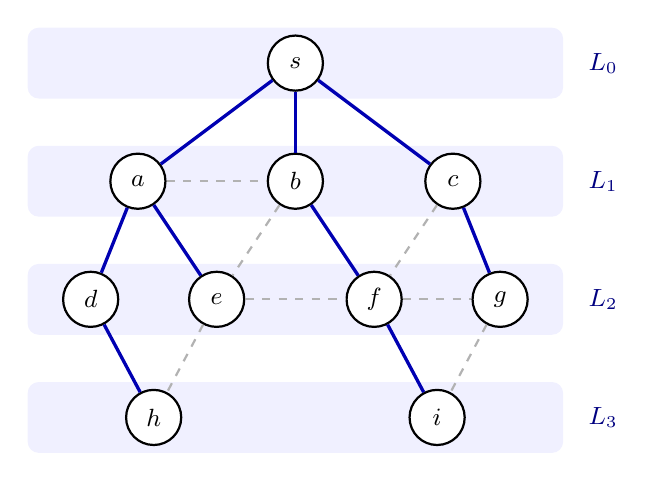
\begin{tikzpicture}[
  vertex/.style={circle, draw, thick, fill=white, minimum size=7mm, inner sep=0pt, font=\small},
  tree/.style={very thick, blue!70!black},
  other/.style={thick, gray!60, dashed},
]
  \foreach \d in {0,...,3} {
    \fill[blue!6, rounded corners] (-3.4,-1.5*\d-0.45) rectangle (3.4,-1.5*\d+0.45);
    \node[font=\small, blue!50!black, anchor=west] at (3.6,-1.5*\d) {$L_\d$};
  }
  \node[vertex] (s) at (0,0) {$s$};
  \node[vertex] (a) at (-2,-1.5) {$a$};
  \node[vertex] (b) at (0,-1.5) {$b$};
  \node[vertex] (c) at (2,-1.5) {$c$};
  \node[vertex] (d) at (-2.6,-3) {$d$};
  \node[vertex] (e) at (-1,-3) {$e$};
  \node[vertex] (f) at (1,-3) {$f$};
  \node[vertex] (g) at (2.6,-3) {$g$};
  \node[vertex] (h) at (-1.8,-4.5) {$h$};
  \node[vertex] (i) at (1.8,-4.5) {$i$};
  \foreach \u/\v in {a/b, b/e, c/f, e/f, f/g, e/h, g/i}
    \draw[other] (\u) -- (\v);
  \foreach \u/\v in {s/a, s/b, s/c, a/d, a/e, b/f, c/g, d/h, f/i}
    \draw[tree] (\u) -- (\v);
\end{tikzpicture}
